% It is an example file showing how to use the 'sigkddExp.cls' 
% LaTeX2e document class file for submissions to sigkdd explorations.
% It is an example which *does* use the .bib file (from which the .bbl file
% is produced).
% REMEMBER HOWEVER: After having produced the .bbl file,
% and prior to final submission,
% you need to 'insert'  your .bbl file into your source .tex file so as to provide
% ONE 'self-contained' source file.
%
% Questions regarding SIGS should be sent to
% Adrienne Griscti ---> griscti@acm.org
%
% Questions/suggestions regarding the guidelines, .tex and .cls files, etc. to
% Gerald Murray ---> murray@acm.org
%

\documentclass{sigkddExp}

\usepackage{listings}
\usepackage{courier}

\lstset{basicstyle=\small\ttfamily,breaklines=true}
% \lstset{framextopmargin=50pt,frame=bottomline}

\begin{document}
%
% --- Author Metadata here ---
% -- Can be completely blank or contain 'commented' information like this...
%\conferenceinfo{WOODSTOCK}{'97 El Paso, Texas USA} % If you happen to know the conference location etc.
%\CopyrightYear{2001} % Allows a non-default  copyright year  to be 'entered' - IF NEED BE.
%\crdata{0-12345-67-8/90/01}  % Allows non-default copyright data to be 'entered' - IF NEED BE.
% --- End of author Metadata ---

% \title{High Performance MapReduce-First Cluster Computing: Design and Applications in Data Mining}
\title{Blaze: Simplified High Performance Cluster Computing}
%\subtitle{[Extended Abstract]
% You need the command \numberofauthors to handle the "boxing"
% and alignment of the authors under the title, and to add
% a section for authors number 4 through n.
%
% Up to the first three authors are aligned under the title;
% use the \alignauthor commands below to handle those names
% and affiliations. Add names, affiliations, addresses for
% additional authors as the argument to \additionalauthors;
% these will be set for you without further effort on your
% part as the last section in the body of your article BEFORE
% References or any Appendices.

\numberofauthors{5}
%
% You can go ahead and credit authors number 4+ here;
% their names will appear in a section called
% "Additional Authors" just before the Appendices
% (if there are any) or Bibliography (if there
% aren't)

% Put no more than the first THREE authors in the \author command
%%You are free to format the authors in alternate ways if you have more 
%%than three authors.

\author{
%
% The command \alignauthor (no curly braces needed) should
% precede each author name, affiliation/snail-mail address and
% e-mail address. Additionally, tag each line of
% affiliation/address with \affaddr, and tag the
%% e-mail address with \email.
\alignauthor Junhao Li \\
       \affaddr{Department of Physics}\\
       \affaddr{Cornell University}\\
       \affaddr{Ithaca, New York, USA}\\
       \email{jl2922@cornell.edu}
\alignauthor Hang Zhang\\
       \affaddr{Department of Electrical and Computer Engineering}\\
       \affaddr{Cornell University}\\
       \affaddr{Ithaca, New York, USA}\\
       \email{hz459@cornell.edu}
}
% \additionalauthors{Additional authors: John Smith (The Th{\o}rvald Group,
% email: {\texttt{jsmith@affiliation.org}}) and Julius P.~Kumquat
% (The Kumquat Consortium, email: {\texttt{jpkumquat@consortium.net}}).}
% \date{30 July 1999}
\maketitle
\begin{abstract}

MapReduce and its variants significantly simplifies cluster computing.
However, many data mining tasks are compute intensive rather than data intensive, and keeping the flexibility of MapReduce while achieving the speed of hand-optimized parallel codes can be difficult.
We present Blaze, a C++ library that makes it easy to develop high performance data parallel softwares.
Blaze is the foundation of Arrow, a new quantum chemistry software that is used in several top research groups and is even faster than other hand-optimized softwares on similar methods.
At the core of Blaze are two sets of features: distributed data containers and the MapReduce function.
% The MapReduce function provides a high performance implementation of performing MapReduce on an input container and saves the results to a mutable output container.
To enable the MapReduce function to run efficiently, Blaze introduces several performance-oriented improvements, including eager reduction, fast serialization, and hash-based shuffle.
Blaze also automatically applies special optimizations for cases where the resulting data container has a small fixed key range, which is common in data mining.
The combination of a simple interface and these performance optimizations makes Blaze an easy-to-use high performance cluster computing library for data mining and similar workflows.
We apply Blaze to several common data mining tasks, including word frequency count, pagerank, k-means, expectation maximization (Gaussian mixture model), and nearest neighbors search.
Blaze outperforms Apache Spark on in-memory computations by an order of magnitude on average and scales almost linearly in performance with the number of nodes.
% In addition, Blaze only uses MapReduce and two utility functions in its implementation while Spark uses more than 20 different parallel primitives in its built-in implementation.


% Over the past decade, MapReduce has revolutionized cloud data processing.
% From our everyday Google searches to advanced business intelligence tools, many cloud services have been rewritten into or created with MapReduce operations to take advantage of the highly-scalable and well-encapsulated MapReduce infrastructures.
% However, previous MapReduce implementations have not taken speed into account seriously.
% This paper presents a design of a High Performance MapReduce-First in-memory cluster computing library called Blaze.
% We redesign both the MapReduce algorithm and implementation from groud-up for in-memory use cases and introduce several performance-oriented improvements, including fast serialization, sort separation, and eager reduction.
% We apply Blaze to several common data mining tasks, including word count, pagerank, k-means, expectation maximization, and nearest neighbors search.
% Blaze scales out almost linearly on these tasks and outperforms in-memory Spark by up to 10 times while using 90\% less memory on average.

\end{abstract}

\section{Introduction}
\cite{dean2008mapreduce,chambers2010flumejava,dean2010mapreduce,zaharia2010spark,zaharia2016apache,davidson2013optimizing,xin2013graphx,meng2016mllib,shanahan2015large,ene2011fast}
Writing parallel programs to take advantage of large computing clusters is a hard task.
MapReduce significantly simplifies this task by providing a high-level abstraction to users and taking care of the low-level operations, such as distributing workloads and comminicating between machines, internally.


MapReduce is a data processing paradigm where we first map each element of the input data to one or more key-value pairs using a map function and then reduce all the pairs with the same key by an associative reduce function to get a single key-value pair for each unique key.

This simple paradigm involves deep design considerations. MapReduce operations can be stacked together to describe most cloud applications, from the search engine that we use everyday to advanced analysis procedures in professional business intelligence solutions. MapReduce implementations, such as Hadoop and Spark, provide developers with well-encapsulated classes that are robust and scalable, so that developers can focus more on their applications. At the time of this writing, MapReduce and its variants are being used in all the major tech companies, serving billions users around the world.

Although widely-used, most MapReduce implementations focus on their capability rather than the performance. Hadoop MapReduce stores all the intermediate results to persistence storage devices, which enables it to handle extremely large datasets but severely limits the performance. Spark provides in-memory MapReduce which can outperform Hadoop by one to two orders of magnitude. However, Spark almost keeps the original MapReduce algorithm which is designed for spinning disks and have not seriously considered performance optimization when the data fits into the memory.

For in-memory MapReduce, the bottleneck shifts from the disks to the amount of computation and the network communication. This study tries to alleviate these new bottlenecks and build a highly-optimized MapReduce library from ground up.

The contributions of this study are listed as follows:

We design and implement fast serialization to achieve higher performance on encoding and decoding and smaller sizes for encoded messages. This reduces the inter-node communication cost.

1. We introduce sort separation, which removes the sort step from MapReduce because many MapReduce jobs don't care about the order of the keys. The sort is replaced with a non-blocking distributed hash table that we design specifically for MapReduce, which reduces the total time complexity of MapReduce from O(nlogn) to O(n). For cases that we do care about the order of the keys, we can further apply the native sort function or use some special parallel sorting libraries.

2. We introduce eager reduction, which tries to perform reduction right after applying the map function. This reduces the memory requirement of MapReduce so that we can use in-memory MapReduce on larger datasets. It also further reduces the inter-node communication cost.

3. We incorporate the improvements above as well as various small improvements and build Blaze, which is a blazing fast MapReduce library that can outperform Spark by 5x on common MapReduce tasks. Similar to Spark, it also supports reusing working datasets for multiple MapReduce operations.

\begin{figure}
  \begin{center}
  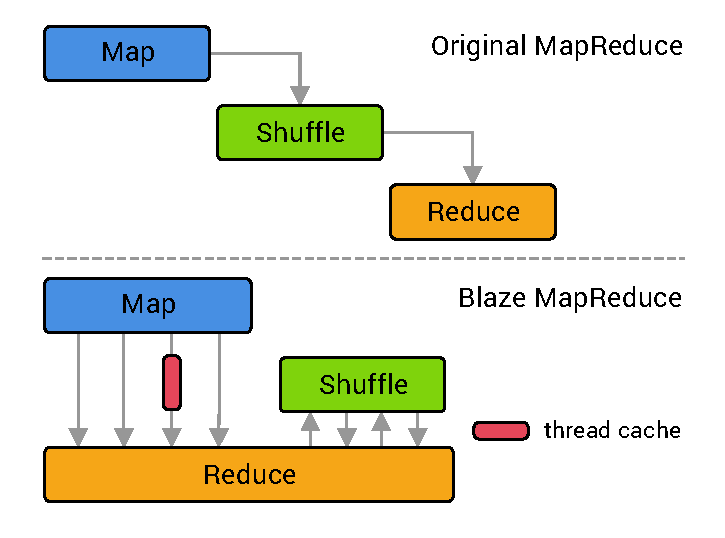
\includegraphics[width=0.9\linewidth]{mrDiff.eps}
  \end{center}
  \vspace{-0.5cm}
  \caption{Hamiltonian matrix construction time for a copper atom in a cc-pVTZ basis. Hamiltonian construction is the performance bottleneck in the variational stage.
%This figure shows that Fast SHCI's new Hamiltonian construction algorithm is an order of magnitude faster than SHCI and several orders of magnitude faster than brute force (loop over each pair of determinants).}
Hamiltonian construction in our improved SHCI algorithm is an order of magnitude faster than in
our original SHCI algorithm, and several orders of magnitude faster than the faster of the two brute force
approaches (loop over each pair of determinants).
Also shown are the number of nonzero elements in the Hamiltonian, scaled so that the first point coincides with
the first point of the improved SHCI CPU time.}
  \label{fig:mrdiff}
\end{figure}

\section{The Blaze Library}


\subsection{Distributed Containers}

\subsection{MapReduce}

\section{Applications}

\section{Related Works}

\section{Conclusion}

MPI/OpenMP has extremely high performance and can outperform Spark/Scala on its most proficient task by almost 300\%.

For cases where we do not care about fault tolerance and only cares about performance or costs, MPI/OpenMP may be a much better choice than Spark. This also includes most offline data analysis use cases, such as business intelligence, where the running time of a task is usually much less than a million core hours. The MTBF (mean time between failures) on modern hardware is on the scale of one million core hours, so the failure rate for these tasks should be extremely low even without fault tolerance, and in the case of a rare failure, we can simply run the task multiple times and as long as it succeeds before the fourth try, we are still likely to get the results faster than using Spark.


% This paragraph will end the body of this sample document.
% Remember that you might still have Acknowledgements or
% Appendices; brief samples of these
% follow.  There is still the Bibliography to deal with; and
% we will make a disclaimer about that here: with the exception
% of the reference to the \LaTeX\ book, the citations in
% this paper are to articles which have nothing to
% do with the present subject and are used as
% examples only.
%\end{document}  % This is where a 'short' article might terminate

%ACKNOWLEDGEMENTS are optional
\section{Acknowledgements}
This work is supported by the U.S. National Science Foundation (NSF) grant ACI-1534965 and the Air Force Office of Scientific Research (AFOSR) grant FA9550-18-1-0095.
We also thank professor Cyrus Umrigar for the helpful suggestions for the paper.

% This section is optional; it is a location for you
% to acknowledge grants, funding, editing assistance and
% what have you.  In the present case, for example, the
% authors would like to thank Gerald Murray of ACM for
% his help in codifying this \textit{Author's Guide}
% and the \textbf{.cls} and \textbf{.tex} files that it describes.

%
% The following two commands are all you need in the
% initial runs of your .tex file to
% produce the bibliography for the citations in your paper.
\bibliographystyle{abbrv}
\bibliography{sigproc}  % sigproc.bib is the name of the Bibliography in this case
% You must have a proper ".bib" file
%  and remember to run:
% latex bibtex latex latex
% to resolve all references
%
% ACM needs 'a single self-contained file'!
%
%APPENDICES are optional
% SIGKDD: balancing columns messes up the footers: Sunita Sarawagi, Jan 2000.
% \balancecolumns
\appendix
%Appendix A
\section{Word frequency count}
In this section, we provide the source code of a common example in MapReduce, which is to count the number of occurrences of each unique word in an input file.
We save the results to a distributed hash map, which can be used for further processing.

\begin{lstlisting}
#include <blaze/blaze.h>
#include <iostream>

int main(int argc, char** argv) {
  blaze::util::init(argc, argv);
  
  // Load file into distributed container.
  auto lines =
      blaze::util::load_file("filepath...");

  // Define mapper function.
  const auto& mapper = [&](
      const size_t,  // Line id.
      const std::string& line,
      const auto& emit) {
    // Split line into words.
    std::stringstream ss(line);
    std::string word;
    while (getline(ss, word, ' ')) {
      emit(word, 1);
    }
  };

  // Define target hash map.
  blaze::DistHashMap<std::string, size_t> words;

  // Perform mapreduce.
  blaze::mapreduce<
      std::string, std::string, size_t>(
          lines, mapper, "sum", words);
    
  // Output number of unique words.
  std::cout << words.size() << std::endl;
  
  return 0;
}
\end{lstlisting}

\section{Monte Carlo Pi Estimation}

In this example, we present a MapReduce implementation of the Monte Carlo $\pi$ estimation.

\begin{lstlisting}
#include <blaze/blaze.h>
#include <iostream>

int main(int argc, char** argv) {
  blaze::util::init(argc, argv);
  
  const size_t N_SAMPLES = 1000000;

  // Define source.
  blaze::DistRange<size_t> samples(0, N_SAMPLES);

  // Define mapper.
  const auto& mapper = 
      [&](const size_t, const auto& emit) {
    // Random function in std is not thread safe.
    double x = blaze::random::uniform();
    double y = blaze::random::uniform();
    if (x * x + y * y < 1) {
      // Map to points within circle to key 0.
      emit(0, 1);
    }
  };

  // Define target.
  std::vector<size_t> count(1);  // {0}

  // Perform MapReduce.
  blaze::mapreduce<size_t, size_t>(
      samples, mapper, "sum", count);

  std::cout << 4.0 * count[0] / N_SAMPLES
      << std::endl;
  
  return 0;
}
\end{lstlisting}

In conventional MapReduce implementations, mapping big data onto a single key is usually not efficient and consumes large amount of memory during the map phase.
Hence, in practice, people usually hand-code parallel for loops in such situations.

However, by using Blaze, the above code will have similar memory consumption and achieve similar performance as a hand-optimized parallel for loops.
In short, Blaze frees users from dealing with low level data communications while ensuring the high performance.

% That's all folks!
\end{document}